% ============================================================
%  Samenvatting: Eindige Elementen Gebaseerd Ontwerp (EEGO)
%  Gegenereerd op basis van cursusmateriaal + examenanalyse
% ============================================================
\documentclass[a4paper,10pt]{article}

\usepackage[dutch]{babel}
\usepackage[T1]{fontenc}
\usepackage[utf8]{inputenc}
\usepackage[margin=1.8cm]{geometry}
\usepackage{amsmath,amssymb}
\usepackage{graphicx}
\usepackage{float}
\usepackage{booktabs}
\usepackage{enumitem}
\usepackage[expansion=false]{microtype}
\usepackage{multicol}
\usepackage{xcolor}
\usepackage{tcolorbox}
\usepackage{hyperref}
\usepackage{array}
\usepackage{tabularx}
\usepackage{caption}

\tcbuselibrary{skins,breakable}

% ---- kleurboxen ----
\newtcolorbox{exambox}[1][]{colback=yellow!15,colframe=orange!70!black,
  fonttitle=\bfseries\small, title=#1, breakable, before skip=4pt, after skip=4pt}
\newtcolorbox{formulebox}[1][]{colback=blue!8,colframe=blue!50!black,
  fonttitle=\bfseries\small, title=#1, breakable, before skip=4pt, after skip=4pt}
\newtcolorbox{warningbox}[1][]{colback=red!8,colframe=red!60!black,
  fonttitle=\bfseries\small, title=#1, breakable, before skip=4pt, after skip=4pt}

\setlength{\parindent}{0pt}
\setlength{\parskip}{3pt}
\setlist{noitemsep, topsep=2pt}

\captionsetup{font=small, labelfont=bf, skip=3pt}

\title{\textbf{Samenvatting EEGO}\\
  \large Eindige Elementen Gebaseerd Ontwerp\\
  \small KU Leuven --- op basis van examens 2015--2026}
\author{Claude Sonnet 4.6}
\date{2025-2026}

\begin{document}
\maketitle
\tableofcontents
\newpage

% ================================================================
\section{FEM-basisconcepten \& Pre/Post-processing}
% ================================================================

Het eindige-elementenprogramma werkt in drie fases:
\begin{itemize}
  \item \textbf{Pre-processing}: geometrie vereenvoudigen (CAD-cleaning), mesh genereren, randvoorwaarden opleggen.
  \item \textbf{Processing}: PDE's omzetten naar lineair stelsel $[K]\{\tilde{q}\} = \{\tilde{F}\}$, oplossen.
  \item \textbf{Post-processing}: resultaten interpreteren, verificatie en validatie.
\end{itemize}

\begin{exambox}[Validatie vs.\ Verificatie --- VEELGEVRAAGD]
\textbf{Validatie}: is het model een goede representatie van de realiteit? (jij iets mis?)\\
\textbf{Verificatie}: heeft de computer correct gerekend, zijn de numerieke/discretisatiefouten acceptabel? (computer iets mis?)
\end{exambox}

\textbf{Numerieke fouten:}
\begin{itemize}
  \item \textit{Discretisatiefout}: neemt af bij meer knopen (fijnere mesh).
  \item \textit{Numerieke afrondingsfout}: neemt toe bij meer knopen (grotere matrix inverteren).
\end{itemize}

\textbf{Rekentijd:} CPU-time $\sim (\text{ndof})^3$ voor volle matrix; met bandstructuur: CPU-time $\sim \text{ndof} \cdot \text{hb}^2$.

\begin{formulebox}[Post-processing: verificatie checklist]
\begin{itemize}
  \item Bekijk \textbf{unaveraged} spanningen $\to$ grote sprong = mesh te grof.
  \item Controleer krachtenevenwicht: som aanlegde krachten = som reactiekrachten.
  \item Doe mesh-convergentiestudie (zie \S\ref{sec:mesh}).
  \item Let op singulariteiten bij scherpe hoeken, puntlasten, einde RBE2.
\end{itemize}
\end{formulebox}

% ================================================================
\section{Elementen, Knopen en Vrijheidsgraden}
% ================================================================

Elk type element heeft een vaste set vrijheidsgraden (DOF) per knoop:

\begin{center}
\renewcommand{\arraystretch}{1.3}
\begin{tabular}{lllll}
\toprule
\textbf{Element} & \textbf{Dim} & \textbf{DOF/knoop} & \textbf{Verplaatsingen} & \textbf{Rotaties}\\
\midrule
ROD (truss)   & 1D & 1 (lokaal) / 2 of 3 (globaal) & $u_x$ & geen\\
BEAM (balk)   & 1D & 6 (3D) & $u_x,u_y,u_z$ & $\theta_x,\theta_y,\theta_z$\\
MEMBRAAN      & 2D & 2 (in-plane) & $u_x,u_y$ & geen\\
PLAAT         & 2D & 3 (out-of-plane) & $u_z$ & $\theta_x,\theta_y$\\
SCHIL (shell) & 2D & 5--6 & $u_x,u_y,u_z$ & $\theta_x,\theta_y$ (+$\theta_z$)\\
SOLID (3D)    & 3D & 3 & $u_x,u_y,u_z$ & geen\\
\bottomrule
\end{tabular}
\end{center}

\begin{exambox}[Wanneer welk element?]
\begin{itemize}
  \item \textbf{ROD}: scharnierende trekstangen, vakwerk (alleen axiale kracht).
  \item \textbf{BEAM}: buigende balken, $L/h > 5\text{--}10$ (Bernoulli geldig).
  \item \textbf{MEMBRAAN}: dunne platen belast \emph{in} het vlak (plane stress / plane strain).
  \item \textbf{PLAAT}: dunne platen belast \emph{uit} het vlak (buiging), $L/t > 10$ (Kirchhoff geldig).
  \item \textbf{SCHIL}: combinatie in-plane + buiging (gekromde oppervlakken).
  \item \textbf{SOLID}: als geen van bovenstaande van toepassing is.
\end{itemize}
\end{exambox}

\textbf{Element-orde (p):}
\begin{itemize}
  \item $p=1$ (lineair): 2 knopen per rand; spanning constant binnen element.
  \item $p=2$ (kwadratisch): 3 knopen per rand (midknoop); spanning lineair binnen element. Beter voor spanningsconcentraties, maar hogere rekentijd.
\end{itemize}

\textbf{Element-vorm:} 2D $\to$ TRIA (3/6 knopen) of QUAD (4/8 knopen); 3D $\to$ TET of HEX.\\
QUAD/HEX zijn nauwkeuriger dan TRIA/TET; TRIA/TET beter voor complexe geometrieën.

\begin{figure}[H]
  \centering
  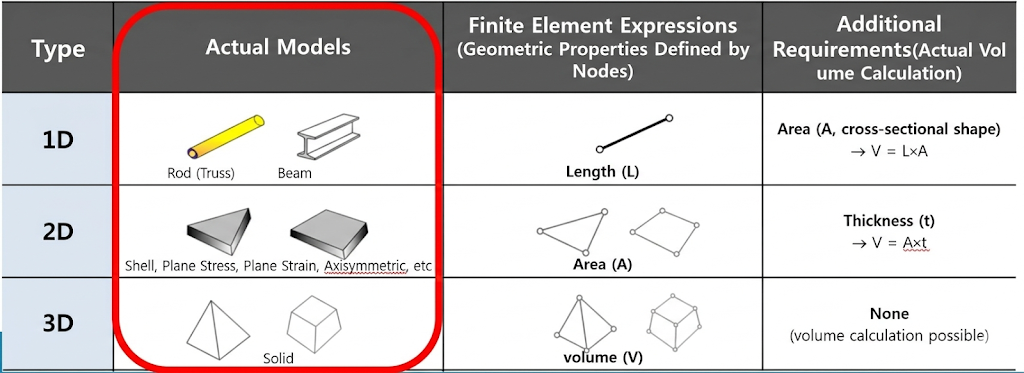
\includegraphics[width=0.75\textwidth]{elementtypetabel.png}
  \caption{Overzicht elementtypen}
\end{figure}

% ================================================================
\section{Vormfuncties (Shape Functions)}
% ================================================================

\begin{exambox}[Wat zijn vormfuncties? --- VEELGEVRAAGD]
Vormfuncties $N_i(x,y,z)$ interpoleren de continue veldvariabele $\hat{q}$ binnenin een element vanuit de knoopwaarden $\{\tilde{q}\}$:
\[
  \hat{q}(x,y,z) = [N]\{\tilde{q}\} = \sum_i N_i \tilde{q}_i
\]
\textbf{Eigenschappen:}
\begin{itemize}
  \item $N_i = 1$ bij eigen knoop $i$; $N_i = 0$ bij alle andere knopen.
  \item $\sum_i N_i = 1$ (partitie van eenheid).
  \item Polynomiale functies; orde bepaalt hoe goed de benadering is.
\end{itemize}
\end{exambox}

\subsection*{1D Lineaire Vormfuncties (ROD, p=1)}

Voor een staaf van knoop 1 ($x=0$) tot knoop 2 ($x=L$):
\[
  N_1(x) = 1 - \frac{x}{L}, \qquad N_2(x) = \frac{x}{L}
\]
\[
  \hat{u}(x) = N_1 \tilde{u}_1 + N_2 \tilde{u}_2
\]
Spanning (rek = afgeleide van verplaatsing, verliest 1 orde!):
\[
  \hat{\epsilon} = \frac{d\hat{u}}{dx} = \frac{\tilde{u}_2 - \tilde{u}_1}{L} = \text{const.} \quad \Rightarrow \quad \hat{\sigma} = E\hat{\epsilon}
\]

\begin{warningbox}[Orde verlies bij differentiëren]
Een lineaire verplaatsing ($p=1$) geeft een constante spanning ($p=0$). Kwadratische elementen ($p=2$) geven een lineaire spanning. Gebruik $p=2$ wanneer je nauwkeurige spanningen nodig hebt.
\end{warningbox}

\subsection*{2D Vormfuncties (TRIA3, lineair)}

Voor een rechthoekig driehoekig element (knopen A$(0,0)$, B$(L_x,0)$, C$(0,L_y)$):
\[
  N_A = 1 - \frac{x}{L_x} - \frac{y}{L_y}, \quad N_B = \frac{x}{L_x}, \quad N_C = \frac{y}{L_y}
\]

\subsection*{Hoeveel vormfuncties heeft een element?}
Aantal vormfuncties = aantal knopen per element. Elke knoop geeft 1 vormfunctie. Een TRIA3 heeft 3 VF, een QUAD4 heeft 4 VF, enz.

\begin{exambox}[Aantal VF \& Matrix-afmetingen (TRIA3 membraan vs.\ plaat)]
\textbf{TRIA3 Membraan} (2 DOF/knoop: $u_x, u_y$):
  3 VF, $[N]$: $2{\times}6$, $[B]$: $3{\times}6$, $[E]$: $3{\times}3$ (plane stress/strain), $[k]$: $6{\times}6$.\\[2pt]
\textbf{TRIA3 Plaat} (3 DOF/knoop: $u_z, \theta_x, \theta_y$):
  9 VF (van hogere orde!), $[N]$: $1{\times}9$, $[B]$: $3{\times}9$, $[E]$: $3{\times}3$ (Kirchhoff), $[k]$: $9{\times}9$.\\
  NB: plaat gebruikt \emph{altijd} vlakke spanningstoestand (door Kirchhoff: $\sigma_z=0$ door dunne-plaat-aanname).
\end{exambox}

\begin{figure}[H]
  \centering
  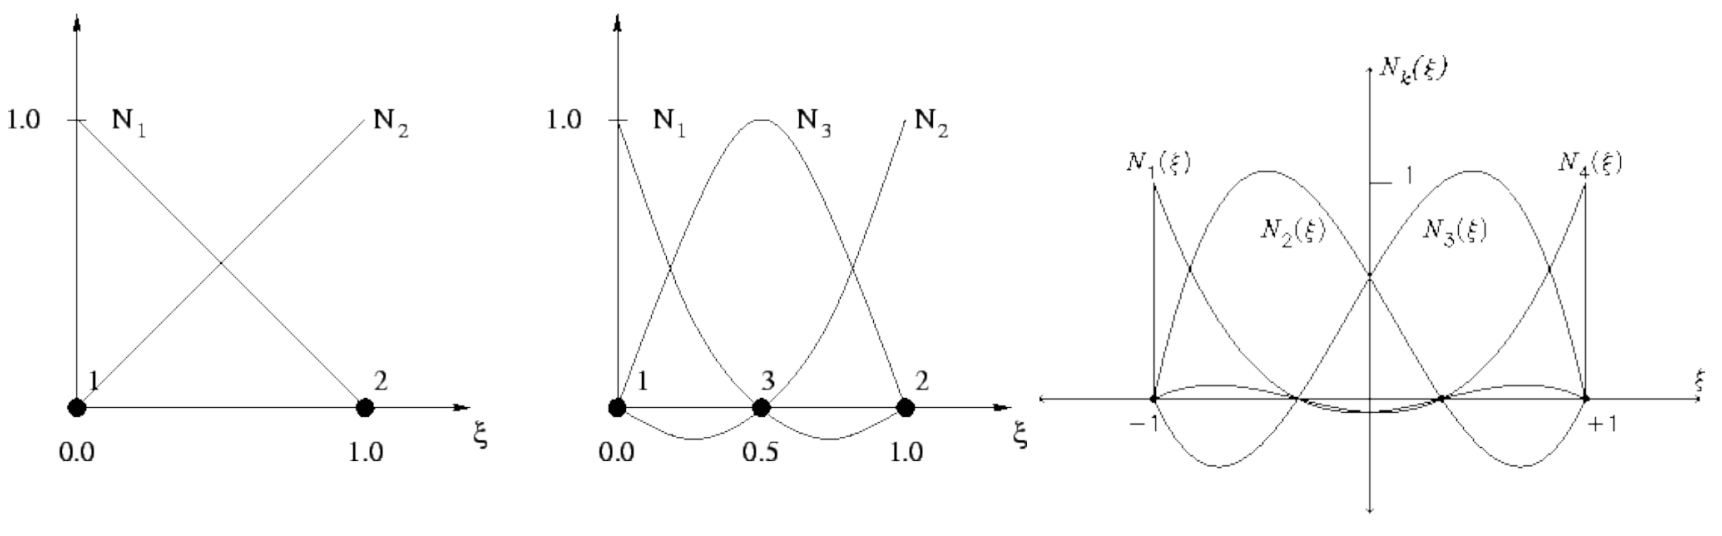
\includegraphics[width=0.8\textwidth]{vormfunctiesvisueel.png}
  \caption{Vormfuncties 1D: lineair ($p=1$), kwadratisch ($p=2$), kubisch ($p=3$)}
\end{figure}

% ================================================================
\section{Randvoorwaarden (Boundary Conditions)}
% ================================================================

\begin{exambox}[3 types randvoorwaarden --- VEELGEVRAAGD]
\textbf{1. Essentieel (Dirichlet / $\Gamma_E$):} opgelegde veldvariabele $\tilde{q} = \bar{q}$.\\
  $\to$ Verplaatsing/rotatie vastleggen (inklemming, scharnier, roloplegging).\\
  $\to$ Bij oplossen: rij \& kolom schrappen uit $[K]$.\\[4pt]
\textbf{2. Natuurlijk (Neumann / $\Gamma_N$):} opgelegde afgeleide $\frac{\partial\tilde{q}}{\partial n} = \bar{f}$.\\
  $\to$ Krachten/momenten (structureel), warmteflux (thermisch).\\
  $\to$ Verschijnt rechtstreeks in rechterlid $\{\tilde{F}\}$.\\[4pt]
\textbf{3. Gemengd (Robin / $\Gamma_M$):} $\alpha\tilde{q} + \beta\frac{\partial\tilde{q}}{\partial n} = \bar{s}$.\\
  $\to$ Verende ondersteuning: $F_{\text{veer}} + k\cdot u = 0$ $\Rightarrow$ veerstijfheid $k$ komt bij diagonaal van $[K]$.\\
  $\to$ Niet-lineair: progressieve veer (stijfheid neemt toe met vervorming); iteratief oplossen.
\end{exambox}

\textbf{Implementatie verende randvoorwaarde (gemengd):}
\[
  [K]\{\tilde{q}\} = \{\tilde{F}\} \quad \to \quad ([K] + [K_{\text{veer}}])\{\tilde{q}\} = \{\tilde{F}\} + \{\tilde{F}_{\text{pretension}}\}
\]
De veerstijfheid $k$ wordt eenvoudig opgeteld bij de overeenkomstige diagonaalelement van $[K]$.

\textbf{Scharnier vs.\ roloplegging vs.\ inklemming:}
\begin{itemize}
  \item Scharnier: $u_x = 0$, $u_y = 0$ (2D); alle translaties = 0 (3D).
  \item Roloplegging: 1 translatie vrij, loodrechte translatie = 0.
  \item Inklemming: alle translaties en rotaties = 0.
\end{itemize}

\textbf{Symmetrie:} Met symmetrierandvoorwaarden kan je je model halveren (of vierendelen): verplaatsing loodrecht op symmetrievlak = 0, rotaties in het symmetrievlak = 0.

% ================================================================
\section{Globale Stijfheidsmatrix \& Knoopnummering}
% ================================================================

\subsection*{Assemblage van de globale stijfheidsmatrix}

De globale matrix $[K]$ wordt opgebouwd door de elementstijfheidsmatrices $[k_e]$ op de juiste positie (op basis van knoopnummers) bij elkaar op te tellen.

\begin{figure}[H]
  \centering
  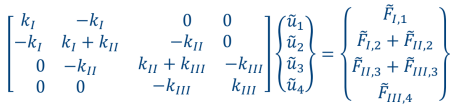
\includegraphics[width=0.6\textwidth]{globalestijfheidsmatrixopgeteld.png}
  \caption{Assemblage van 3 elementen tot globale $[K]$}
\end{figure}

$[K]$ is singulier (niet inverteerbaar) zolang het model vrij in de ruimte kan bewegen (rigid body motion) $\to$ essentiële randvoorwaarden zijn verplicht!

\subsection*{Skyline en Halve Bandbreedte}

\begin{formulebox}[Halve Bandbreedte (hb) --- VEELGEVRAAGD]
\[
  \text{hb} = \max_e \left[ \frac{\text{ndof}}{\text{node}} \cdot (\max_e(\Delta\text{NodeID}) + 1) \right]
\]
Met $\Delta\text{NodeID}$ = maximaal knoopnummerverschil \emph{binnen} één element.\\
CPU-time $\sim \text{ndof} \cdot \text{hb}^2$: \textbf{kleine hb $\to$ snelle berekening!}\\[4pt]
\textbf{Optimale nummering}: geef knopen die aan hetzelfde element vastzitten, nummers zo dicht mogelijk bij elkaar. Nummer bij voorkeur kortste richting van de mesh.
\end{formulebox}

\begin{figure}[H]
  \centering
  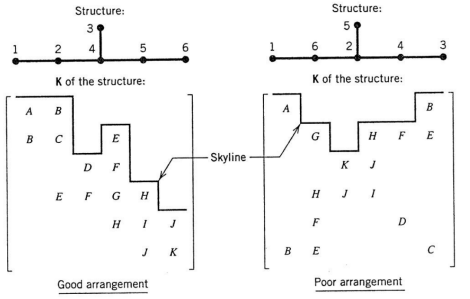
\includegraphics[width=0.7\textwidth]{skylinesbeidegevallen.png}
  \caption{Twee identieke modellen: links goede nummering (hb=3), rechts slechte nummering (hb=6). Rekentijdverhouding: $3^2 : 6^2 = 1:4$.}
\end{figure}

% ================================================================
\section{Elementstijfheidsmatrices: Directe Methode}
% ================================================================

\subsection*{1D ROD Element}

\begin{formulebox}[Elementstijfheidsmatrix ROD]
\[
  [k_e] = \frac{AE}{L}\begin{bmatrix} 1 & -1 \\ -1 & 1 \end{bmatrix}
  \qquad \Leftrightarrow \qquad
  \begin{bmatrix} k & -k \\ -k & k \end{bmatrix}\begin{Bmatrix}\tilde{u}_1\\\tilde{u}_2\end{Bmatrix} = \begin{Bmatrix}\tilde{F}_1\\\tilde{F}_2\end{Bmatrix}
\]
Vereiste invoer: doorsnede $A$, E-modulus $E$ (lengte $L$ uit mesh).
\end{formulebox}

\subsection*{1D BEAM Element (zuivere buiging, Bernoulli)}

\begin{exambox}[Bernoulli vs.\ Timoshenko --- VEELGEVRAAGD]
\textbf{Bernoulli:} dwarsdoorsnede blijft vlak \emph{en loodrecht} op de neutrale as na vervorming.\\
$\Rightarrow$ Schuifvervorming $\gamma_{xy} = 0$ (verwaarloosbaar). Geldig voor slanke balken: $L/h > 5\text{--}10$.\\[3pt]
\textbf{Timoshenko:} dwarsdoorsnede blijft vlak maar \emph{niet loodrecht}. Neemt schuifvervorming mee. Beter voor korte/dikke balken.
\end{exambox}

Relatie Bernoulli: $\theta_y = \frac{\partial u_z}{\partial x}$ (rotatie = afgeleide van doorbuiging).

DOF per knoop (buiging 2D): $\tilde{u}_z$ (doorbuiging) en $\tilde{\theta}_y$ (rotatie) $\to$ 4 DOF totaal voor 2-knoopselement.

\begin{formulebox}[4$\times$4 Elementstijfheidsmatrix BEAM (buiging)]
\[
  [k_e] = \frac{EI}{L^3}\begin{bmatrix}
    12 & 6L & -12 & 6L \\
    6L & 4L^2 & -6L & 2L^2 \\
    -12 & -6L & 12 & -6L \\
    6L & 2L^2 & -6L & 4L^2
  \end{bmatrix}
  \qquad \text{volgorde: } \tilde{u}_{z1},\tilde{\theta}_{y1},\tilde{u}_{z2},\tilde{\theta}_{y2}
\]
Vereiste invoer: $E$, buigtraagheidsmoment $I_y$ (en $I_z$ in 3D), dwarsdoorsnede voor schuifgebied.
\end{formulebox}

\textbf{Hoe brekende spanning berekenen (BEAM)?}
\[
  \hat{\sigma}_x(x,z) = E\hat{\epsilon}_x = E\left(-z\frac{d^2\hat{u}_z}{dx^2}\right)
\]
waarbij $z$ = afstand tot neutrale as. Spanning is lineair over de doorsnede (maximaal aan de uiterste vezel).\\
Orde van nauwkeurigheid: spanning is van orde $p-1 = 1$ (want buiging vereist 2e afgeleide van $p=3$ VF $\to$ lineaire spanning). De breekvorm is kubisch ($p=3$) voor een lineair beam-element.

\subsection*{Transformatiematrix voor schuinstaande 1D Elementen}

Wanneer een 1D element \emph{niet} parallel loopt aan de globale assen (hoek $\alpha$ met x-as):
\[
  [k_{\text{globaal}}] = [T]^T [k_{\text{lokaal}}] [T]
\]

\begin{formulebox}[Transformatiematrix voor ROD in 2D]
\[
  [T] = \begin{bmatrix} c & s & 0 & 0 \\ -s & c & 0 & 0 \\ 0 & 0 & c & s \\ 0 & 0 & -s & c \end{bmatrix}, \quad c = \cos\alpha,\; s = \sin\alpha
\]
\end{formulebox}

\begin{exambox}[Transformatiematrix ROD vs.\ BEAM?]
De transformatiematrix voor een ROD en een BEAM is \emph{niet} hetzelfde.\\
Bij een BEAM komen er ook rotaties bij (extra rijen/kolommen), en er zijn 3 assen in 3D.\\
De structuur is wel gelijkaardig: rotatiematrix $[T]$ met $c$ en $s$ termen.
\end{exambox}

% ================================================================
\section{Energie-gebaseerde Methode (Matrix Flow)}
% ================================================================

\begin{exambox}[Matrix Flow --- VEELGEVRAAGD]
\textbf{Het principe:} externe arbeid = interne elasticiteitsenergie $\Rightarrow$ algemene stijfheidsmatrix.
\[
  \frac{1}{2}\{\tilde{u}\}^T\{\tilde{F}\} = \int_{\Omega_e} \frac{1}{2}\{\hat{\epsilon}\}^T\{\hat{\sigma}\}\,dV
\]

\textbf{Stap 1:} Verplaatsing interpoleren: $\{\hat{u}\} = [N]\{\tilde{u}\}$\\[2pt]
\textbf{Stap 2:} Rek bepalen (afgeleiden van verplaatsing): $\{\hat{\epsilon}\} = [\partial]\{\hat{u}\} = [\partial][N]\{\tilde{u}\} = [B]\{\tilde{u}\}$\\[2pt]
\textbf{Stap 3:} Spanning via Hooke: $\{\hat{\sigma}\} = [E]\{\hat{\epsilon}\} = [E][B]\{\tilde{u}\}$\\[4pt]
\textbf{Resultaat:}
\[
  \boxed{[k_e] = \int_{\Omega_e} [B]^T [E] [B]\,dV}
\]
\end{exambox}

\begin{figure}[H]
  \centering
  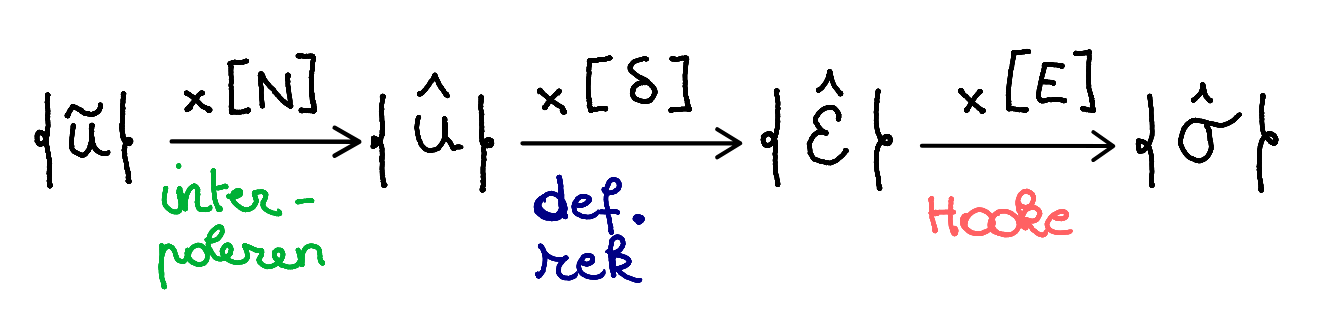
\includegraphics[width=0.75\textwidth]{spanningbepalen.png}
  \caption{Matrix Flow: van knoopverplaatsingen naar spanning ($[N] \to [B] \to [E]$)}
\end{figure}

\textbf{Betekenis van de matrices:}
\begin{itemize}
  \item $[N]$: vormfunctiematrix; hangt af van elementgeometrie.
  \item $[B] = [\partial][N]$: strain-displacement matrix; afgeleiden van VF.
  \item $[E]$: constitutieve matrix (materiaalwet, Hooke); hangt af van $E, \nu$.
\end{itemize}

\textbf{Verificatie voor 1D ROD:} invullen van $N_1=1-x/L$, $N_2=x/L$ geeft $[B] = [-1/L \; 1/L]$, $[E] = E$:
\[
  [k_e] = \int_0^L \begin{Bmatrix}-1/L\\1/L\end{Bmatrix} E \begin{bmatrix}-1/L&1/L\end{bmatrix} A\,dx = \frac{AE}{L}\begin{bmatrix}1&-1\\-1&1\end{bmatrix} \checkmark
\]

\textbf{Matrixafmetingen voor TRIA3 Membraan:}
$[B]$: $3\times6$ (3 reken = $\epsilon_x,\epsilon_y,\gamma_{xy}$; 6 DOF); $[E]$: $3\times3$; $[k_e]$: $6\times6$.

% ================================================================
\section{2D Elementen: Membraan, Plaat, Schil}
% ================================================================

\subsection*{Membraan (in-plane)}

\textbf{Rekcomponenten (2D):} $\hat{\epsilon}_x = \frac{\partial\hat{u}_x}{\partial x}$, $\hat{\epsilon}_y = \frac{\partial\hat{u}_y}{\partial y}$, $\hat{\gamma}_{xy} = \frac{\partial\hat{u}_x}{\partial y}+\frac{\partial\hat{u}_y}{\partial x}$.

\begin{exambox}[Plane Stress vs.\ Plane Strain --- VEELGEVRAAGD]
\textbf{Vlakke spanningstoestand (Plane Stress)}: $\sigma_z = 0$; vrije rek in $z$-richting.\\
Toepassingen: \textbf{dunne platen} belast in het vlak (bv.\ dunne membraanplaat).
\[
  [E]_{\text{stress}} = \frac{E}{1-\nu^2}\begin{bmatrix}1&\nu&0\\\nu&1&0\\0&0&\frac{1-\nu}{2}\end{bmatrix}
\]

\textbf{Vlakke vervormingstoestand (Plane Strain)}: $\epsilon_z = 0$; geen rek in $z$-richting.\\
Toepassingen: \textbf{lange/dikke structuren} (dammen, buizen, tunnels) ver van de uiteinden.
\[
  [E]_{\text{strain}} = \frac{E}{(1+\nu)(1-2\nu)}\begin{bmatrix}1-\nu&\nu&0\\\nu&1-\nu&0\\0&0&\frac{1-2\nu}{2}\end{bmatrix}
\]
\end{exambox}

\begin{figure}[H]
  \centering
  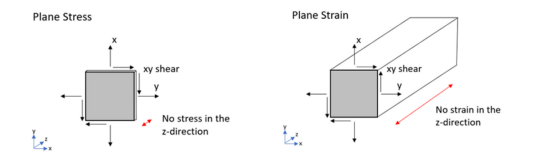
\includegraphics[width=0.72\textwidth]{plainstressvsplainstrain.png}
  \caption{Plane stress (dun/kort) vs.\ plane strain (lang/dik)}
\end{figure}

\textbf{Vereiste invoer membraan:} $E$, $\nu$, dikte $t$ (want $dV = t\cdot dA$).

\subsection*{Plaatelement (out-of-plane buiging)}

\textbf{Kirchhoff-aanname:} dwarsdoorsnede blijft vlak en loodrecht op het middenvlak na vervorming (2D-equivalent van Bernoulli). Geldig voor dunne platen: $L/t > 10$.

DOF per knoop: $u_z$, $\theta_x$, $\theta_y$ (geen in-plane!) $\to$ TRIA3 plaat heeft $3\times3=9$ DOF.

De [E]-matrix voor een plaat is \emph{altijd plane stress} (vlakke spanningstoestand), want de plaat is dun ($\sigma_z \approx 0$).

\begin{exambox}[Verschil Membraan vs.\ Plaat (TRIA3)]
\begin{tabular}{lll}
 & \textbf{Membraan} & \textbf{Plaat} \\
DOF/knoop & 2 ($u_x, u_y$) & 3 ($u_z, \theta_x, \theta_y$) \\
Totale DOF & 6 & 9 \\
$[N]$-grootte & $2\times6$ & $1\times9$ \\
$[B]$-grootte & $3\times6$ & $3\times9$ \\
$[E]$-grootte & $3\times3$ & $3\times3$ \\
$[k]$-grootte & $6\times6$ & $9\times9$ \\
VF orde & 1 (lineair) & 3 (kubisch) \\
Belasting & in-plane & uit-het-vlak (buiging) \\
\end{tabular}
\end{exambox}

\subsection*{Schilelement (Shell)}

Shell = membraan + plaat $\Rightarrow$ 5 of 6 DOF/knoop. Gebruikt voor gekromde dunne oppervlakken.

\subsection*{Isoparametrische Elementen \& Jacobiaan}

Willekeurige elementvormen worden gemapped naar een standaard $\xi\eta$-element ($-1 \le \xi,\eta \le 1$):
\[
  [k_e] = \int_{-1}^{+1}\int_{-1}^{+1} [B]^T[E][B]\det([J])\,d\xi\,d\eta
\]
$[J]$ = Jacobiaanmatrix (schaalt en roteert van lokaal naar globaal stelsel). Vereist convex element; anders is mapping niet uniek.

% ================================================================
\section{3D Elementen}
% ================================================================

\textbf{DOF per knoop:} 3 translaties ($u_x, u_y, u_z$), geen rotaties.

\textbf{Rekcomponenten:} 6 componenten ($\epsilon_x, \epsilon_y, \epsilon_z, \gamma_{xy}, \gamma_{yz}, \gamma_{xz}$) $\Rightarrow$ $[B]$: $6\times(3n)$; $[E]$: $6\times6$.

\textbf{3D Wet van Hooke --- materiaalmatrix} $[E]$:
\[
\{\hat{\sigma}\} = \begin{Bmatrix}\sigma_x\\\sigma_y\\\sigma_z\\\tau_{xy}\\\tau_{yz}\\\tau_{xz}\end{Bmatrix}
= \frac{E}{(1+\nu)(1-2\nu)}
\begin{bmatrix}
1-\nu & \nu & \nu & 0 & 0 & 0\\
\nu & 1-\nu & \nu & 0 & 0 & 0\\
\nu & \nu & 1-\nu & 0 & 0 & 0\\
0&0&0&\frac{1-2\nu}{2}&0&0\\
0&0&0&0&\frac{1-2\nu}{2}&0\\
0&0&0&0&0&\frac{1-2\nu}{2}
\end{bmatrix}
\begin{Bmatrix}\epsilon_x\\\epsilon_y\\\epsilon_z\\\gamma_{xy}\\\gamma_{yz}\\\gamma_{xz}\end{Bmatrix}
\]

\textbf{Wanneer 3D?} Als alle dimensies van vergelijkbare orde zijn. Nadeel: véél DOF, hoge rekentijd.

\begin{figure}[H]
  \centering
  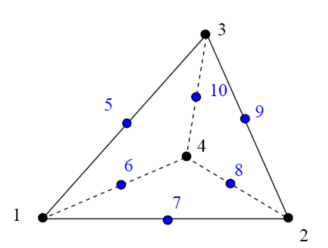
\includegraphics[width=0.45\textwidth]{3Delemennttt.png}
  \caption{3D elementen: tet4, tet10, hex8, hex20}
\end{figure}

% ================================================================
\section{Hybride Meshes \& Multi-Point Constraints (MPC)}
% ================================================================

\subsection*{Problemen bij combineren van elementen}

\begin{itemize}
  \item \textbf{Verschillende DOFs}: bv.\ beam (met rotaties) aan membraan (zonder rotaties) $\to$ incompatibel.
  \item \textbf{Geometrische gaten (gaps)}: 1D mesh ligt op neutrale as, 2D op midsurface $\to$ gaten bij assemblage.
  \item \textbf{Verschillende ordes}: kubische VF (beam/plaat) naast lineaire VF (membraan) $\to$ scheur.
\end{itemize}

\subsection*{Multi-Point Constraints (MPC)}

\begin{exambox}[Wat zijn MPC's? --- VEELGEVRAAGD]
Een MPC is een wiskundige vergelijking die de verplaatsing van \textbf{slave}-knopen koppelt aan \textbf{master}-knopen:
\[
  \{\tilde{u}_{\text{slave}}\} = [C_{\text{MPC}}]\{\tilde{u}_{\text{master}}\}
\]
3 toepassingen:
\begin{enumerate}
  \item Koppelen van elementen met \emph{verschillende DOFs} (beam aan membraan).
  \item Koppelen van elementen met \emph{verschillende VF-ordes} (kwadratisch aan lineair).
  \item \emph{Glue}: verbinden van niet-overlappende meshes met verschillende knooppositie.
\end{enumerate}
\end{exambox}

\textbf{Voorbeeld 1: beam aan membraan} (knoop 1 = beam, knopen A,B = membraan, afstand $a$):
\[
  \begin{Bmatrix}\tilde{u}_{xA}\\\tilde{u}_{yA}\\\tilde{u}_{xB}\\\tilde{u}_{yB}\end{Bmatrix} =
  \begin{bmatrix}1&0&0\\0&1&-a\\1&0&0\\0&1&a\end{bmatrix}
  \begin{Bmatrix}\tilde{u}_{x1}\\\tilde{u}_{y1}\\\tilde{\theta}_{z1}\end{Bmatrix}
\]

\textbf{Voorbeeld 2: kwadratisch element naast lineair element} (midknoop 2 slave, hoekknopen 1 en 3 master):
\[
  \tilde{u}_{x2} = 0.5\tilde{u}_{x1} + 0.5\tilde{u}_{x3}, \quad \tilde{u}_{y2} = 0.5\tilde{u}_{y1} + 0.5\tilde{u}_{y3}
\]
\textbf{Regel:} het element met de \emph{laagste orde} is altijd de master.

\subsection*{RBE2 vs. RBE3}

\begin{exambox}[RBE2 vs.\ RBE3 --- VEELGEVRAAGD]
\textbf{RBE2} (Rigid Body Element type 2):
\begin{itemize}
  \item Perfect stijf: slave-knopen volgen master exact (onderlinge afstand verandert niet).
  \item Gebruikt voor: stijve verbindingen, lasnaad simulatie, geometrische gaten dichten.
  \item VOORZICHTIG: introduceert onrealistische stijfheid; eindigt in singulariteiten aan de rand.
\end{itemize}
\textbf{RBE3} (Rigid Body Element type 3):
\begin{itemize}
  \item Geen stijfheid toegevoegd: verdeelt een puntlast (op master) over slave-knopen via gewogen gemiddelde van de VF.
  \item Gebruikt voor: belasting uitsmeert over meerdere knopen (bv.\ pijp op plaat).
\end{itemize}
\textbf{Hoofdverschil:} RBE2 = stijf koppeling (verplaatsing voorschrijven), RBE3 = krachtverdeling.
\end{exambox}

\begin{figure}[H]
  \centering
  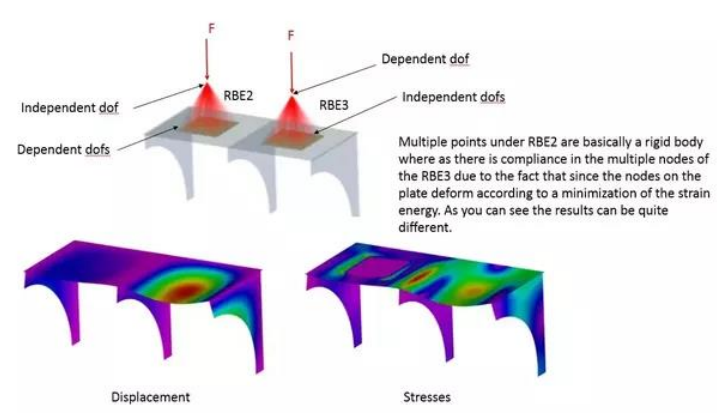
\includegraphics[width=0.55\textwidth]{RBE2VSRBE3PLAAT.png}
  \caption{RBE2 (links) vs.\ RBE3 (rechts): stijve verbinding vs.\ krachtverdeling}
\end{figure}

\textbf{RBE2 vs.\ Glue:}
\begin{itemize}
  \item RBE2: behoudt fysieke afstand (gap) $\to$ correcte hefboomwerking.
  \item Glue (= MPC type 3): trekt meshes wiskundig samen $\to$ verlies van fysieke offset.
\end{itemize}

% ================================================================
\section{Praktische Overwegingen: Mesh Design}\label{sec:mesh}
% ================================================================

\subsection*{Mesh Generatie}
\begin{itemize}
  \item \textbf{Automatisch}: snel maar geen controle; overal gelijke elementen.
  \item \textbf{Mapped (interactief)}: lokale verfijning bij spanningsconcentraties; aanbevolen.
  \item \textbf{Manueel}: maximale controle, tijdrovend; gebruik extrude/revolve/sweep om 2D mesh naar 3D te trekken.
\end{itemize}

\textbf{Mesh Seeding}: zaadje planten op randen = aantal knopen opgeven per rand.

\textbf{Mesh Biasing}: knopen lokaal dichter bij spanningsconcentraties (bv.\ gaten, inkepingen). Bias = $\Delta X_{\max}/\Delta X_{\min}$.

\subsection*{Element Kwaliteit}

\begin{warningbox}[Slechte elementen vermijden]
\begin{itemize}
  \item Gebruik QUAD boven TRIA waar mogelijk: nauwkeuriger, minder elementen nodig.
  \item Vermijd niet-convexe elementen (hoek $> 180^\circ$): Jacobiaan wordt negatief.
  \item Mesh-transitie: overgang fijn-grof niet te abrupt; gebruik transitie-elementen.
  \item Cirkels: min 12-20 elementen voor $< 1\text{--}5\%$ geometrische fout.
\end{itemize}
\end{warningbox}

\begin{figure}[H]
  \centering
  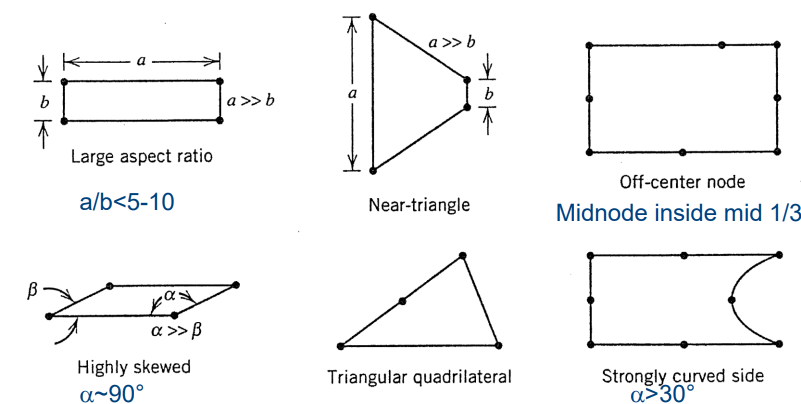
\includegraphics[width=0.6\textwidth]{afbeelding_poor_elements.png}
  \caption{Slechte vs.\ goede elementvormen}
\end{figure}

\subsection*{Mesh Convergentie vs.\ Mesh Sensitiviteit}

\begin{exambox}[Mesh Convergentie vs.\ Sensitiviteit --- VEELGEVRAAGD]
\textbf{Mesh Convergentiestudie}: verfijn de mesh (meer elementen, $h$-refinement) $\to$ bekijk hoe het resultaat convergeert naar een stabiele waarde. Analyseert \textbf{discretisatiefouten}.\\[2pt]
\textbf{Mesh Sensitiviteitsstudie}: varieer de elementvorm/-grootte bij \emph{gelijk} aantal DOF $\to$ bekijk hoe gevoelig het resultaat is aan de mesh. Analyseert zowel \textbf{discretisatie-} als \textbf{numerieke fouten}.\\[4pt]
\textbf{Verfijningsmethodes:}\\
$h$-refinement: kleinere elementen (meer knopen). $p$-refinement: hogere orde VF ($p=1 \to p=2$). $r$-refinement: knopen herpositioneren.\\[2pt]
Kwadratische ($p=2$) elementen convergeren sneller dan lineaire ($p=1$).
\end{exambox}

\begin{figure}[H]
  \centering
  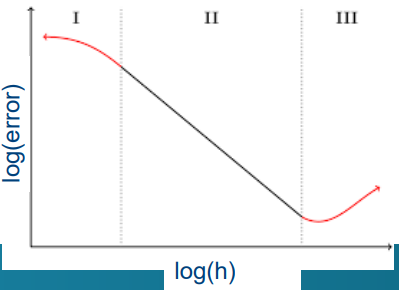
\includegraphics[width=0.60\textwidth]{afbeelding_mesh_convergence.png}
  \caption{Mesh convergentiegrafiek: stijgend dan afvlakkend naar exacte waarde. Lineair trager dan kwadratisch.}
\end{figure}

\subsection*{Automatische Mesh Adaptatie}

De software berekent lokale fout (op basis van spanningssprongen) $\to$ verfijnt automatisch daar waar de fout te groot is $\to$ herberekent $\to$ herhaalt tot convergentie.

\subsection*{Singulariteiten}

Bij scherpe hoeken, puntlasten en einde van RBE2-elementen: $\sigma \to \infty$ bij mesh-verfijning (geen convergentie!).\\
\textbf{Oplossing}: voeg een afrondingsstraal (fillet) toe; dan convergeert $\sigma$ wel naar een eindige waarde.

\begin{figure}[H]
  \centering
  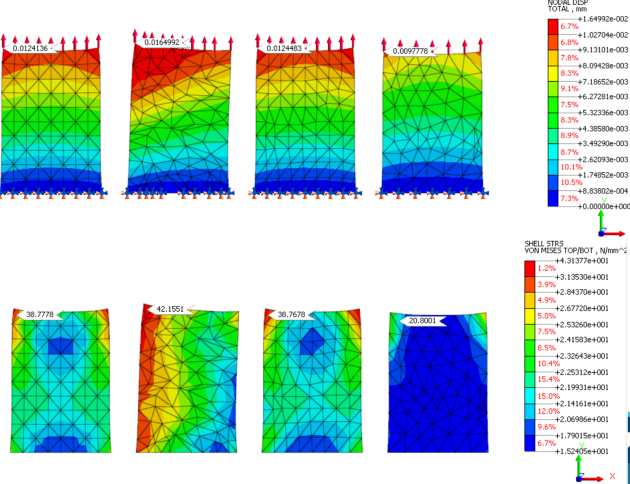
\includegraphics[width=0.5\textwidth]{afbeelding_singularities_illustration.png}
  \caption{Singulariteit bij scherpe hoek: spanning divergeert bij verfijning}
\end{figure}

% ================================================================
\section{Post-processing: Spanningen en Verificatie}
% ================================================================

\subsection*{Spanningsberekening}

\[
  \{\hat{\sigma}\} = [E][B]\{\tilde{u}\}
\]

Spanningen worden intern berekend in Gauss-punten (integratiepunten) en geëxtrapoleerd naar knopen.

\begin{exambox}[Elemental vs.\ Nodal; Averaged vs.\ Unaveraged]
\textbf{Elemental}: 1 waarde per element (zwaartepunt); mist piekspanningen aan randen.\\
\textbf{Nodal (corner data)}: waarden geëxtrapoleerd naar knopen; toont werkelijke pieken.\\[4pt]
\textbf{Unaveraged}: ruwe waarden; toont spanningssprongen tussen elementen $\to$ gebruik voor verificatie!\\
\textbf{Averaged}: gemiddeld over aangrenzende elementen; gladde plot $\to$ gebruik voor presentatie, maar \emph{verbergt fouten}.\\[4pt]
\textbf{Regel:} grote spanningssprong bij unaveraged $\Rightarrow$ mesh verfijnen.
\end{exambox}

\subsection*{Von Mises Spanning}

\[
  \sigma_{VM} = \frac{1}{\sqrt{2}}\sqrt{(\sigma_x-\sigma_y)^2 + (\sigma_y-\sigma_z)^2 + (\sigma_z-\sigma_x)^2 + 6(\tau_{xy}^2+\tau_{yz}^2+\tau_{zx}^2)}
\]

\begin{warningbox}[Von Mises alleen voor ductiel materiaal!]
Von Mises = maat voor vloeibegin. Voor brosse materialen: gebruik hoofdspanningen. Vergelijk bij validatie altijd met dezelfde spanningscomponent als de analytische methode (bv.\ $\sigma_x$ voor buiging via Navier).
\end{warningbox}

\subsection*{Verificatie van de Simulatie}

\begin{enumerate}
  \item Krachtenevenwicht: som aanlegde krachten $\approx$ som reactiekrachten (afwijking = numerieke fout).
  \item Spanningssprongen (unaveraged): klein $\to$ mesh OK; groot $\to$ verfijnen.
  \item Mesh-convergentiestudie: resultaat stabil bij verfijning?
  \item Vergelijk met analytische of experimentele referentiewaarden.
\end{enumerate}

% ================================================================
\section{Snel-naslagkaart: Examen-topics}\label{sec:snel}
% ================================================================

\begin{center}
\renewcommand{\arraystretch}{1.4}
\begin{tabular}{p{5cm}p{9cm}}
\toprule
\textbf{Onderwerp} & \textbf{Kernpunt}\\
\midrule
Vormfuncties & $N_i=1$ bij knoop $i$, 0 elders; $\sum N_i=1$; 1 VF per knoop\\
Aantal VF & = aantal knopen per element\\
Stijfheidsmatrix algemeen & $[k] = \int [B]^T[E][B]\,dV$\\
Stijfheidsmatrix ROD & $\frac{AE}{L}\begin{bmatrix}1&-1\\-1&1\end{bmatrix}$\\
Stijfheidsmatrix BEAM & $\frac{EI}{L^3}[12,6L,-12,6L;\ldots]$ (zie \S6)\\
Bandbreedte & $\text{hb} = \max_e[\frac{\text{ndof}}{\text{node}}(\Delta\text{NodeID}+1)]$; CPU $\sim \text{ndof}\cdot\text{hb}^2$\\
Plane stress & dun object, $\sigma_z=0$; $[E] = \frac{E}{1-\nu^2}[\ldots]$\\
Plane strain & lang object, $\epsilon_z=0$; $[E] = \frac{E}{(1+\nu)(1-2\nu)}[\ldots]$\\
Plaat-[E] & altijd plane stress (Kirchhoff, $L/t>10$)\\
Bernoulli & $\gamma_{xy}=0$; geldig $L/h>5\text{--}10$\\
MPC & slave = $[C]$ master; 3 types: DOF, orde, glue\\
RBE2 & stijf, koppeling, geen massa; pas op singulariteit\\
RBE3 & geen stijfheid, krachtverdeling; VF nodig\\
Singulariteit & scherpe hoek/puntlast/RBE2-einde; fillet oplossing\\
Mesh convergentie & meer knopen $\to$ discrfout $\downarrow$; unaveraged stress\\
Von Mises & ductiel materiaal; niet vergelijken met $\sigma_x$ analytisch\\
Verificatie & krachtenevenwicht + spanningssprong + convergentie\\
\bottomrule
\end{tabular}
\end{center}

\end{document}
